\documentclass[a4paper,11pt,fleqn]{article}
\usepackage{fullpage}
\usepackage{pdfpages}
\usepackage{amsmath}
\usepackage[dutch]{babel}
\usepackage{float}
\setlength{\mathindent}{0cm}
\usepackage{fancyhdr}
\setlength{\headheight}{15.2pt}
\pagestyle{fancy}
\fancyhf{}
\lhead{\leftmark}
\rhead{\thepage}

\hyphenation{gegeven}
\hyphenation{kruisproducten}
\hyphenation{zeker}

\begin{document}

%Titelblad
\begin{center}

% Upper part of the page. The '~' is needed because \\
% only works if a paragraph has started.
\includegraphics[width=0.30\textwidth]{./kuleuven}~\\[1cm]

\textsc{\LARGE KU Leuven}\\[1.5cm]


% Title
\HRule \\[0.4cm]
{ \huge \bfseries TOEGEPASTE MECHANICA 2 \\
Deel Dynamica CASE 2014-2015 \\[0.4cm] }

\HRule \\[1.5cm]
\vspace{5cm}
% Author and supervisor
\noindent
\begin{flushleft} \large
Pieter \textsc{Van Damme}\\
Wouter \textsc{Van Gansbeke}\\
Lennert \textsc{Vanmunster}\\
Ruben \textsc{Verhulst}
\end{flushleft}


\vfill

% Bottom of the page
{\large \today}

\end{center}

\newpage
%ToC
\tableofcontents
\thispagestyle{plain}
\newpage

%Transformatiematrices
\section{Transformatiematrices}
\thispagestyle{plain}

\subsection{Van het $x'y'z'$-assenstelstel naar het $xyz$-assenstelsel}
Het $x'y'z'$ assenstelsel wordt bekomen door het $xyz$-assenstelsel te roteren met een hoek $\alpha$ rond de x-as. De omgekeerde transformatie draait dus met een negatieve hoek $\alpha$ rond de x-as. Het $x''y''z''$-assenstelsel heeft dezelfde ori\"entatie als het $x'y'z'$-assenstelsel. Hun transformatiematrices zijn daarom hetzelfde.

\begin{figure}[H]
\centering
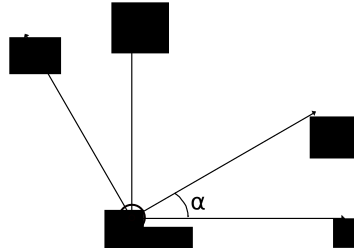
\includegraphics[scale=0.5]{x'y'z'.pdf}
\caption{Het $x'y'z'$-assenstelsel}
\end{figure}

\begin{equation*}
R^{x'y'z' \rightarrow xyz}=
  \begin{bmatrix}
    1 & 0 & 0\\
    0 & \cos(\alpha) & -\sin{\alpha}\\ 
    0 & \sin{\alpha} & \cos(\alpha)\
    \end{bmatrix}
\end{equation*}



\subsection{Van het $x'''y'''z'''$-assenstelsel naar het $x''y''z''$-assenstelsel}
Het $x'''y'''z'''$-assenstelsel wordt bekomen door het $x''y''z''$-assenstelsel te roteren met een hoek $\beta$ rond de $y''$-as. De transformatiematrix draait dus met een negatieve hoek $\beta$ rond de $y'''$-as. Deze transformatiematrix kan ook gebruikt worden om coördinaten naar het $x'y'z'$-assenstelsel te converteren. De ori\"entatie van het $x'y'z'$-assentstelsel en van het $x''y''z''$-assenstelsel is immers hetzelfde.

\begin{figure}[H]
\centering
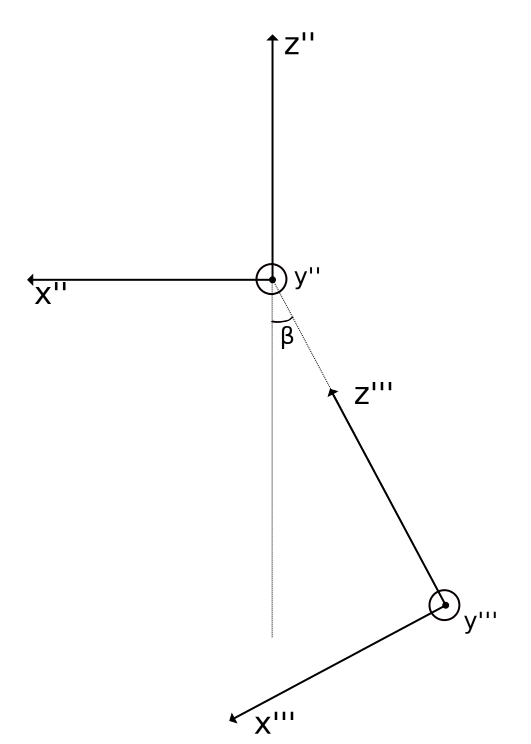
\includegraphics[scale=0.35]{x'''y'''z'''.pdf}
\caption{Het $x'''y'''z'''$-assenstelsel}
\end{figure}

\begin{equation*}
R^{x'''y'''z''' \rightarrow x''y''z''}=
  \begin{bmatrix}
    \cos(\beta) & 0 & sin(\beta)\\
    0 & 1 & 0\\ 
    -\sin(\beta) & 0 & \cos(\beta)\
    \end{bmatrix}
\end{equation*}

Voor de omgekeerde transformatie wordt deze matrix ge\"inverteerd.
\begin{equation*}
R^{x''y''z'' \rightarrow x'''y'''z'''}=
  \begin{bmatrix}
    \cos(\beta) & 0 & -sin(\beta)\\
    0 & 1 & 0\\ 
    \sin(\beta) & 0 & \cos(\beta)\
    \end{bmatrix}
\end{equation*}


\subsection{Van het $x'''y'''z'''$-assenstelsel naar het $xyz$-assenstelsel}
Om van het $x'''y'''z'''$-assenstelsel naar het $xyz$-assenstelsel te gaan, worden de vorige twee berekende transformatiematrices met alkaar vermenigvuldigd. Eerst worden de $x'''y'''z'''$-co\"ordinaten getransformeerd naar het $x''y''z''$-assenstelsel. Vervolgens worden ze omgezet naar het $xyz$-assenstelsel.
\begin{equation*}
\begin{split}
R^{x'''y'''z''' \rightarrow xyz} & =R^{x'''y'''z''' \rightarrow x''y''z''}R^{x'y'z' \rightarrow xyz} \\
&=
  \begin{bmatrix}
      1 & 0 & 0\\
      0 & \cos(\alpha) & -\sin{\alpha}\\ 
      0 & \sin{\alpha} & \cos(\alpha)\
      \end{bmatrix}
  \begin{bmatrix}
      \cos(\beta) & 0 & sin(\beta)\\
      0 & 1 & 0\\ 
      -\sin(\beta) & 0 & \cos(\beta)\
      \end{bmatrix} \\
&=
  \begin{bmatrix}
      \cos(\beta) & 0 & \sin(\beta)\\
      \sin(\alpha)\sin(\beta) & \cos(\alpha) & -\sin(\alpha)\cos(\beta)\\
      -\cos(\alpha)\sin(\beta) & \sin(\alpha) & \cos(\alpha)\cos(\beta)\  
      \end{bmatrix}
\end{split}
\end{equation*}

\newpage
%Deel kinematica
\newpage
\section{Kinematica}
\thispagestyle{plain}

\subsection{Vraag 1}
%Inleidende tekst
Om de ogenblikkelijke totale rotatiesnelheidsvector $\overrightarrow{\omega}_{w}$ te bepalen worden de drie afzonderlijke rotatiesnelheidsvectoren uitgedrukt in het wereldassenstelsel en vervolgens opgeteld.
\begin{equation*}
\overrightarrow{\omega}_{w}=R^{x'y'z' \rightarrow xyz}\,\overrightarrow{\omega}_{g}'+R^{x'y'z' \rightarrow xyz}\,\overrightarrow{\omega}_{i}'+R^{x'''y'''z''' \rightarrow xyz}\,\overrightarrow{\omega}_{w}'''
\end{equation*}



Deze termen worden nu afzonderlijk bepaald.
%omega_g
\begin{equation*}
\begin{split}
R^{x'y'z' \rightarrow xyz}\,\overrightarrow{\omega}_{g}'
&=	  \begin{bmatrix}
      1 & 0 & 0\\
      0 & \cos(\alpha) & -\sin{\alpha}\\ 
      0 & \sin{\alpha} & \cos(\alpha)\
      \end{bmatrix}
      \begin{bmatrix}
      0\\
      0\\
      \omega_{g}\
      \end{bmatrix}     
&=	  \begin{bmatrix}
      0\\
      -\sin{\alpha}\,\omega_{g}\\
      \cos(\alpha)\,\omega_{g}\
      \end{bmatrix}
\end{split}
\end{equation*}

%omega_i
\begin{equation*}
\begin{split}
R^{x'y'z' \rightarrow xyz}\,\overrightarrow{\omega}_{g}'
&=	  \begin{bmatrix}
      1 & 0 & 0\\
      0 & \cos(\alpha) & -\sin{\alpha}\\ 
      0 & \sin{\alpha} & \cos(\alpha)\
      \end{bmatrix}
      \begin{bmatrix}
      0\\
      \omega_{i}\\
      0\
      \end{bmatrix}     
&=	  \begin{bmatrix}
      0\\
      \cos{\alpha}\,\omega_{i}\\
      \sin(\alpha)\,\omega_{i}\
      \end{bmatrix}
\end{split}
\end{equation*}

%omega_w
\begin{equation*}
\begin{split}
R^{x'''y'''z''' \rightarrow xyz}\,\overrightarrow{\omega}_{w}'''
&=	  \begin{bmatrix}
      \cos(\beta) & 0 & \sin(\beta)\\
      \sin(\alpha)\sin(\beta) & \cos(\alpha) & -\sin(\alpha)\cos(\beta)\\
      -\cos(\alpha)\sin(\beta) & \sin(\alpha) & \cos(\alpha)\cos(\beta)\  
      \end{bmatrix}
      \begin{bmatrix}
      -\omega_{w}\\
      0\\
      0\
      \end{bmatrix}
&=    \begin{bmatrix}
      -\cos(\beta)\,\omega_{w}\\
      -\sin(\alpha)\sin(\beta)\,\omega_{w}\\
      \cos(\alpha)\sin(\beta)\,\omega_{w}\
      \end{bmatrix}
\end{split}
\end{equation*}

De ogenblikkelijke rotatievector wordt dus weergegeven door door de volgende vergelijking.
\begin{equation*}
\overrightarrow(\omega)_{w}=
\begin{bmatrix}
	-\cos(\beta)\,\omega_{w}\\
	\cos(\alpha)\,\omega_{i} - \sin(\alpha)(\omega_{g}+\sin{\beta}\,\omega_{w})\\
	\sin(\alpha)\,\omega_{i} + \cos(\alpha)(\omega_{g}+\sin{\beta}\,\omega_{w})\
\end{bmatrix}
\end{equation*}

\subsection{Vraag 2}

\subsubsection{De ogenblikkelijke snelheid}
De snelheid van C kan beschouwd worden als de som van de relatieve snelheid van het punt C in het $x'y'z'$-assenstelsel en de snelheid van dat assenstelsel. In dit assenstelsel kan de beweging van C beschouwd worden als een som van rotaties, nl. een rotatie rond het punt A door $\overrightarrow{\omega_{g}}$ en een rotatie rond het punt B door $\overrightarrow{\omega_{i}}$

\begin{equation*}
\overrightarrow{v_{C}}=\overrightarrow{v_{A}}+\overrightarrow{\omega_{g}}\times(\overrightarrow{r_{C}}-\overrightarrow{r_{A}})+\overrightarrow{\omega_{i}}\times(\overrightarrow{r_{C}}-\overrightarrow{r_{B}})
\end{equation*}

Deze termen worden afzonderlijk bepaald.

\begin{equation*}
\begin{split}
\overrightarrow{v_{A}}
&=R^{x'y'z' \rightarrow xyz}
	\begin{bmatrix}
	0\\
	v_v\\
	0
	\end{bmatrix}
&=	\begin{bmatrix}
0\\
v_v\cos(\alpha)\\
v_v\sin(\alpha)\
\end{bmatrix}
\end{split}
\end{equation*}

\begin{equation*}
\begin{split}
\overrightarrow{r_{C}}-\overrightarrow{r_{A}}
&=\begin{bmatrix}
r_{CAx}\\
r_{CAy}\\
r_{CAz}\
\end{bmatrix}
&=R^{x'y'z' \rightarrow xyz}
	\begin{bmatrix}
	l_{1}-l_{3}\sin(\beta)-l_{4}\cos(\beta)\\
	0\\
	l_{2}-l_{3}\cos(\beta)+l_{4}\sin(\beta)\
	\end{bmatrix}
&=	\begin{bmatrix}
	l_{1}-l_{3}\sin(\beta)-l_{4}\cos(\beta)\\
	-\sin(\alpha)(l_{2}-l_{3}\cos(\beta)+l_{4}\sin(\beta))\\
	\cos(\alpha)(l_{2}-l_{3}\cos(\beta)+l_{4}\sin(\beta))\
	\end{bmatrix}
\end{split}
\end{equation*}

\begin{equation*}
\begin{split}
\overrightarrow{\omega_{g}}\times(\overrightarrow{r_{C}}-\overrightarrow{r_{A}})
&=	\begin{vmatrix}
\overrightarrow{e_{x}} & \overrightarrow{e_{y}} & \overrightarrow{e_{z}}\\
\omega_{gx} & \omega_{gy} & \omega_{gz}\\
r_{CAx} & r_{CAy} & r_{Caz}\
\end{vmatrix}
\end{split}
\end{equation*}

\subsection{Vraag 3}
Om de bijdrage van de coriolisversnelling te bepalen kan de volgende formule gebruikt worden. Het $x''y''z''$-assenstelsel wordt als hulpassenstelsel genomen.
\begin{equation*}
\overrightarrow{a_{coriolis}}=-2\,(\overrightarrow{\omega}\times\overrightarrow{v_{rel}})
\end{equation*}

Om de versnelling van het voorwerp te beschrijven, wordt $\omega$ gelijkgesteld aan $\omega_{i}$. Dit is immers de enige rotatie die het punt C uitvoert in het hulpassenstelsel. De relatieve snelheid in dit assenstelsel is de rotatiesnelheid van het assenstelsel, namelijk de rotatiesnelheid van B rond A met $\overrightarrow{\omega_{g}}$. 

\begin{equation*}
\begin{split}
\overrightarrow{\omega}=\overrightarrow{\omega_{i}}
\end{split}
\end{equation*}

\begin{equation*}
\begin{split}
\overrightarrow{v_{rel}}&= \overrightarrow{\omega_{i}}\times(\overrightarrow{r_{C}}-\overrightarrow{r_{B}})
&=	\begin{bmatrix}
	-\omega_{i}\, \left( l_{3}\,\cos \left( \beta \right) -l_{4}\,\sin \left( \beta \right)  \right) \\
	-\omega_{i}\,\sin \left( \alpha \right)  \left( l_{3}\,\sin \left( \beta \right) +l_{4}\,\cos \left( \beta \right) \right) \\
	\omega_{i}\,\cos \left( \alpha \right) \left( l_{3}\,\sin \left( \beta \right) +l_{4}\,\cos \left( \beta\right)  \right) \
\end{bmatrix}
\end{split}
\end{equation*}

\begin{equation*}
\begin{split}
\overrightarrow{a_{coriolis}}&=
\begin{bmatrix}
0\\
2\,\cos \left( \alpha\right) \omega_{g}\,\omega_{i}\, \left( l_{3}\,\cos \left( \beta\right) -l_{4}\,\sin \left( \beta \right)  \right) \\
2\,\sin \left( \alpha \right) \omega_{g}\,\omega_{i}\, \left( l_{3}\,\cos \left( \beta \right) -l_{4}\,\sin \left( \beta \right)  \right) \
\end{bmatrix}
\end{split}
\end{equation*}

\subsection{Vraag 4}
\subsubsection{Ogenblikkelijke snelheid}
Voor het berekenen van de snelheid van D wordt een gelijkaardige methode gebruikt als voor de snelheid van C in deel \ref{snelh_c}. Aangezien D zich niet op het wiel bevindt, heeft de rotatie van het wiel nog steeds geen invloed op de snelheid. De beweging kan dus opnieuw beschreven worden als de som van de translatiesnelheid van het vliegtuig, de rotatiesnelheid rond A en de rotatiesnelheid rond B.

\begin{equation} \label{eq:snelh_d}
\overrightarrow{v_{D}}=\overrightarrow{v_{A}}+\overrightarrow{\omega_{g}}\times(\overrightarrow{r_{D}}-\overrightarrow{r_{A}})+\overrightarrow{\omega_{i}}\times(\overrightarrow{r_{D}}-\overrightarrow{r_{B}})
\end{equation}

%rel plaats D-A
\begin{equation*}
\begin{split}
\overrightarrow{r_{D}}-\overrightarrow{r_{A}}
&=	(\overrightarrow{r_{D}}-\overrightarrow{r_{C}}) + 		(\overrightarrow{r_{C}}-\overrightarrow{r_{A}})\\
&=	R^{x'''y'''z''' \rightarrow xyz}
	\begin{bmatrix}
	\frac{3}{4}l_{4}\\
	0\\
	\frac{1}{4}l_{3}\
	\end{bmatrix}
	+\begin{bmatrix}
	r_{CAx}\\
	r_{CAy}\\
	r_{CAz}\
	\end{bmatrix}\\
&=	\begin{bmatrix}
	-1/4\,l_{4}\,\cos \left( \beta \right) -3/4\,l_{3}\,\sin \left( \beta \right) +l_{1}\\
	%
	3/4\,\sin \left( \beta \right) \sin \left( \alpha \right) l_{4}-1/4\,\cos\left( \beta \right) \sin \left( \alpha \right) l_{3}-\sin \left( \alpha \right)  \left( -l_{3}\,\cos \left( \beta \right) +l_{4}\,\sin\left( \beta \right) +l_{2} \right) \\
	%
	-3/4\,\sin\left( \beta \right) \cos \left( \alpha \right) l_{4}+1/4\,\cos\left( \beta \right) \cos \left( \alpha \right) l_{3}+\cos \left( \alpha \right)  \left( -l_{3}\,\cos \left( \beta \right) +l_{4}\,\sin\left( \beta \right) +l_{2} \right) \
	\end{bmatrix}
\end{split}
\end{equation*}

%kruis omega_g - rel plaats D-A
\begin{equation*}
\begin{split}
\overrightarrow{\omega_{g}}\times(\overrightarrow{r_{D}}-\overrightarrow{r_{A}})
&=	\begin{vmatrix}
	\overrightarrow{e_{x}} & \overrightarrow{e_{y}} & \overrightarrow{e_{z}}\\
	\omega_{gx} & \omega_{gy} & \omega_{gz}\\
	v_{DAx} & v_{DAy} & v_{DAz}\
	\end{vmatrix}
&=	\begin{bmatrix}
	0\\
	%
	-1/4\,\omega_{g}\,\cos\left( \alpha \right)  \left( 3\,l_{3}\,\sin \left( \beta \right) +l_{4}\,\cos \left( \beta \right) -4\,l_{1} \right) \\
	%
	-1/4\,\omega_{g}\,\sin \left( \alpha \right)  \left( 3\,l_{3}\,\sin\left( \beta \right) +l_{4}\,\cos \left( \beta \right) -4\,l_{1}\right) \
	\end{bmatrix}
\end{split}
\end{equation*}

%rel plaats D-B
\begin{equation*}
\begin{split}
\overrightarrow{r_{D}}-\overrightarrow{r_{B}}
&=	(\overrightarrow{r_{D}}-\overrightarrow{r_{C}}) + 		(\overrightarrow{r_{C}}-\overrightarrow{r_{B}})\\
&=	\begin{bmatrix}
	-1/4\,l_{4}\,\cos \left( \beta \right) -3/4\,l_{3}\,\sin \left( \beta \right) \\
	%
	3/4\,\sin\left( \beta \right) \sin \left( \alpha \right) l_{4}-1/4\,\cos\left( \beta \right) \sin \left( \alpha \right) l_{3}-\sin \left( \alpha \right)  \left( -l_{3}\,\cos \left( \beta \right) +l_{4}\,\sin\left( \beta \right)  \right) \\
	%
	-3/4\,\sin \left( \beta \right) \cos \left( \alpha \right) l_{4}+1/4\,\cos \left( \beta\right) \cos \left( \alpha \right) l_{3}+\cos \left( \alpha \right) \left( -l_{3}\,\cos \left( \beta \right) +l_{4}\,\sin \left( \beta\right)  \right) \	
	\end{bmatrix}
\end{split}
\end{equation*}

%kruis omega_i - rel plaats D-B
\begin{equation*}
\begin{split}
\overrightarrow{\omega_{i}}\times(\overrightarrow{r_{D}}-\overrightarrow{r_{B}})
&=	\begin{vmatrix}
	\overrightarrow{e_{x}} & \overrightarrow{e_{y}} & \overrightarrow{e_{z}}\\
	\omega_{ix} & \omega_{iy} & \omega_{iz}\\
	v_{DBx} & v_{DBy} & v_{DBz}\
	\end{vmatrix}
&=	\begin{bmatrix}
	-1/4\,\omega_{i}\, \left( 3\,l_{3}\,\cos\left( \beta \right) -l_{4}\,\sin \left( \beta \right)  \right) \\
	%
	-1/4\,\omega_{i}\,\sin \left( \alpha \right) \left( 3\,l_{3}\,\sin \left( \beta \right) +l_{4}\,\cos \left( \beta\right)  \right) \\
	%
	1/4\,\omega_{i}\,\cos \left( \alpha \right)  \left( 3\,l_{3}\,\sin \left( \beta \right) +l_{4}\,\cos \left( \beta \right)  \right) \
	\end{bmatrix}
\end{split}
\end{equation*}

De totale snelheid van D wordt dus door de volgende gelijkheid gegeven.
\begin{equation*}
\begin{split}
\overrightarrow{v_{D}}
&=	\begin{bmatrix}
	-1/4\,\omega_{i}\, \left( 3\,l_{3}\,\cos\left( \beta \right) -l_{4}\,\sin \left( \beta \right)  \right) \\
	%
	\cos \left( \alpha \right) v_{v}-1/4\,\omega_{g}\,\cos \left( \alpha \right)  \left( 3\,l_{3}\,\sin \left( \beta\right) +l_{4}\,\cos \left( \beta \right) -4\,l_{1} \right) -1/4\,\omega_{i}\,\sin \left( \alpha \right)  \left( 3\,l_{3}\,\sin \left( \beta \right) +l_{4}\,\cos \left( \beta \right)  \right) \\
	%
	\sin \left( \alpha \right) v_{v}-1/4\,\omega_{g}\,\sin \left( \alpha \right)  \left( 3\,l_{3}\,\sin \left( \beta\right) +l_{4}\,\cos \left( \beta \right) -4\,l_{1} \right) +1/4\,\omega_{i}\,\cos \left( \alpha \right)  \left( 3\,l_{3}\,\sin \left( \beta \right) +l_{4}\,\cos \left( \beta \right)  \right) \
	\end{bmatrix}
\end{split}
\end{equation*}

\subsubsection{Ogenblikkelijke versnelling}
Ook voor de ogenblikkelijke versnelling van D wordt een gelijkaardige methode gebruikt als voor C in deel \ref{versn_c}. De vergelijking die hierboven werdt berekend (vgl. \ref{eq:snelh_d}) wordt afgeleid naar de tijd..

\begin{equation}
\begin{split}
\overrightarrow{a_{D}}&=\frac{d\overrightarrow{v_{D}}}{dt}
&=	\overrightarrow{a_{A}} + \frac{d\overrightarrow{\omega_{g}}}{dt}\times(\overrightarrow{r_{D}}-\overrightarrow{r_{A}}) + \overrightarrow{\omega_{g}}\times(\overrightarrow{v_{D}}-\overrightarrow{v_{A}}) + \frac{d\overrightarrow{\omega_i}}{dt}\times(\overrightarrow{r_{D}}-\overrightarrow{r_{B}})+\overrightarrow{\omega_{i}}\times(\overrightarrow{v_{D}}-\overrightarrow{v_{B}})
\end{split}
\end{equation}

Opnieuw worden al deze termen afzonderlijk uitgerekend.

%a_A
\begin{equation*}
\begin{split}
\overrightarrow{a_{A}}
&=	\begin{bmatrix}
	0\\
	a_v\cos(\alpha)\\
	a_v\sin(\alpha)\
	\end{bmatrix}
\end{split}
\end{equation*}

%kruis d_omega_g - rel plaats D-B
\begin{equation*}
\begin{split}
\frac{d\overrightarrow{\omega_{g}}}{dt}\times(\overrightarrow{r_{D}}-\overrightarrow{r_{A}})
&=	\begin{vmatrix}
	\overrightarrow{e_{x}} & \overrightarrow{e_{y}} & \overrightarrow{e_{z}}\\
	\frac{d\overrightarrow{\omega_g}}{dt}_{x} & \frac{d\overrightarrow{\omega_g}}{dt}_{y} & \frac{d\overrightarrow{\omega_g}}{dt}_{z}\\
	r_{DAx} & r_{DAy} & r_{DAz}\
	\end{vmatrix}
&=	\begin{bmatrix}
	0\\
	%
	-1/4\,\alpha_{g}\,\cos\left( \alpha \right)  \left( 3\,l_{3}\,\sin \left( \beta \right) +l_{4}\,\cos \left( \beta \right) -4\,l_{1} \right) \\
	%
	-1/4\,\alpha_{g}\,\sin \left( \alpha \right)  \left( 3\,l_{3}\,\sin\left( \beta \right) +l_{4}\,\cos \left( \beta \right) -4\,l_{1}\right) \
	\end{bmatrix}
\end{split}
\end{equation*}

%kruis omega_g - rel snelh D-B
\begin{equation*}
\begin{split}
\overrightarrow{\omega_{g}}\times(\overrightarrow{v_{D}}-\overrightarrow{v_{A}})
&=	\begin{vmatrix}
	\overrightarrow{e_{x}} & \overrightarrow{e_{y}} & \overrightarrow{e_{z}}\\
	\omega_{gx} & \omega_{gy} & \omega_{gz}\\
	v_{DAx} & v_{DAy} & v_{DAz}\
	\end{vmatrix}
&=	\begin{bmatrix}
	1/4\,{\omega_{g}}^{2} \left( 3\,l_{3}\,\sin\left( \beta \right) +l_{4}\,\cos \left( \beta \right) -4\,l_{1}\right) \\
	%
	1/4\,\cos \left( \alpha \right) \omega_{g}\,\omega_{i}\, \left( l_{4}\,\sin \left( \beta \right) -3\,l_{3}\,\cos \left( \beta \right)  \right) \\
	%
	1/4\,\sin\left( \alpha \right) \omega_{g}\,\omega_{i}\, \left( l_{4}\,\sin\left( \beta \right) -3\,l_{3}\,\cos \left( \beta \right)  \right) \
	\end{bmatrix}
\end{split}
\end{equation*}

%kruis d_omega_i - rel plaats D-B
\begin{equation*}
\begin{split}
\frac{d\overrightarrow{\omega_i}}{dt}\times(\overrightarrow{r_{D}}-\overrightarrow{r_{B}})
&=	\begin{vmatrix}
	\overrightarrow{e_{x}} & \overrightarrow{e_{y}} & \overrightarrow{e_{z}}\\
	\frac{d\overrightarrow{\omega_i}}{dt}_{x} & \frac{d\overrightarrow{\omega_i}}{dt}_{y} & \frac{d\overrightarrow{\omega_i}}{dt}_{z}\\
	r_{DBx} & r_{DBy} & r_{DBz}\
	\end{vmatrix}\\
&=	\begin{bmatrix}
	1/4\,\alpha_{i}\, \left( l_{4}\,\sin \left( \beta \right) -3\,l_{3}\,\cos \left( \beta \right)  \right) \\
	\\
	%
	1/4\,\sin \left( \beta \right) \cos \left( \alpha\right) l_{4}\,\omega_{g}\,\omega_{i}-3/4\,\cos \left( \beta \right) \cos \left( \alpha \right) l_{3}\,\omega_{g}\,\omega_{i}\cdots\\
	\cdots-3/4\,\sin\left( \beta \right) \sin \left( \alpha \right) l_{3}\,\alpha_{i}-1/4\,\cos \left( \beta \right) \sin \left( \alpha \right) l_{4}\,\alpha_{i}\\
	\\
	%
	1/4\,\sin \left( \beta \right) \sin \left( \alpha \right) l_{4}\,\omega_{g}\,\omega_{i}-3/4\,\cos \left( \beta\right) \sin \left( \alpha \right) l_{3}\,\omega_{g}\,\omega_{i}\cdots\\
	\cdots+3/4\,\sin \left( \beta \right) \cos \left( \alpha \right) l_{3}\,\alpha_{i}+1/4\,\cos \left( \beta \right) \cos \left( \alpha \right) l_{4}\,\alpha_{i}\
	\end{bmatrix}
\end{split}
\end{equation*}

%kruis omega_i - rel snelh D-B
\begin{equation*}
\begin{split}
\overrightarrow{\omega_{i}}\times(\overrightarrow{v_{D}}-\overrightarrow{v_{B}})
&=	\begin{vmatrix}
	\overrightarrow{e_{x}} & \overrightarrow{e_{y}} & \overrightarrow{e_{z}}\\
	\omega_{ix} & \omega_{iy} & \omega_{iz}\\
	v_{DBx} & v_{DBy} & v_{DBz}\
	\end{vmatrix}
&=	\begin{bmatrix}
	1/4\,{\omega_{i}}^{2} \left( 3\,l_{3}\,\sin\left( \beta \right) +l_{4}\,\cos \left( \beta \right)  \right) \\
	%
	1/4\,\omega_{i}\,\sin \left( \alpha \right) \left( \sin \left( \beta \right) l_{4}\,\omega_{i}-3\,\cos \left( \beta \right) l_{3}\,\omega_{i}+4\,\sin \left( \alpha \right) \omega_{g}\,l_{2} \right) \\
	%
	-1/4\,\omega_{i}\,\cos \left( \alpha \right)  \left( \sin \left( \beta \right) l_{4}\,\omega_{i}-3\,\cos \left( \beta \right) l_{3}\,\omega_{i}+4\,\sin \left( \alpha\right) \omega_{g}\,l_{2} \right) \
	\end{bmatrix}
\end{split}
\end{equation*}

Dit wordt allemaal opgeteld.

\begin{equation*}
\begin{split}
\overrightarrow{a_{D}}
&=	\begin{bmatrix}
1/4\,{\omega_{g}}^{2} \left( 3\,l_{3}\,\sin\left( \beta \right) +l_{4}\,\cos \left( \beta \right) -4\,l_{1}\right) +1/4\,\alpha_{i}\, \left( l_{4}\,\sin \left( \beta \right) -3\,l_{3}\,\cos \left( \beta \right)  \right)\cdots\\
\cdots +1/4\,{\omega_{i}}^{2}\left( 3\,l_{3}\,\sin \left( \beta \right) +l_{4}\,\cos \left( \beta\right)  \right) \\
\\
%
a_{v}\,\cos \left( \alpha\right) -1/4\,\alpha_{g}\,\cos \left( \alpha \right)  \left( 3\,l_{3}\,\sin \left( \beta \right) +l_{4}\,\cos \left( \beta \right) -4\,l_{1} \right)\cdots\\
\cdots +1/4\,\cos \left( \alpha \right) \omega_{g}\,\omega_{i}\,\left( l_{4}\,\sin \left( \beta \right) -3\,l_{3}\,\cos \left( \beta\right)  \right) +1/4\,\sin \left( \beta \right) \cos \left( \alpha\right) l_{4}\,\omega_{g}\,\omega_{i}\cdots\\
\cdots-3/4\,\cos \left( \beta \right) \cos \left( \alpha \right) l_{3}\,\omega_{g}\,\omega_{i}-3/4\,\sin\left( \beta \right) \sin \left( \alpha \right) l_{3}\,\alpha_{i}\cdots\\
\cdots-1/4\,\cos \left( \beta \right) \sin \left( \alpha \right) l_{4}\,\alpha_{i}+1/4\,\omega_{i}\,\sin \left( \alpha \right)  \left( \sin \left( \beta \right) l_{4}\,\omega_{i}-3\,\cos \left( \beta \right) l_{3}\,\omega_{i}+4\,\sin \left( \alpha \right) \omega_{g}\,l_{2} \right) \\
\\
%
a_{v}\,\sin \left( \alpha \right) -1/4\,\alpha_{g}\,\sin \left( \alpha \right)  \left( 3\,l_{3}\,\sin \left( \beta \right) +l_{4}\,\cos \left( \beta \right) -4\,l_{1} \right)\cdots\\
\cdots +1/4\,\sin \left( \alpha \right) \omega_{g}\,\omega_{i}\, \left( l_{4}\,\sin \left( \beta \right) -3\,l_{3}\,\cos \left( \beta \right) \right) +1/4\,\sin \left( \beta \right) \sin \left( \alpha \right) l_{4}\,\omega_{g}\,\omega_{i}\cdots\\
\cdots-3/4\,\cos \left( \beta \right) \sin\left( \alpha \right) l_{3}\,\omega_{g}\,\omega_{i}+3/4\,\sin \left( \beta \right) \cos \left( \alpha \right) l_{3}\,\alpha_{i}\cdots\\
+1/4\,\cos\left( \beta \right) \cos \left( \alpha \right) l_{4}\,\alpha_{i}-1/4\,\omega_{i}\,\cos \left( \alpha \right)  \left( \sin \left( \beta\right) l_{4}\,\omega_{i}-3\,\cos \left( \beta \right) l_{3}\,\omega_{i}+4\,\sin \left( \alpha \right) \omega_{g}\,l_{2} \right) \
\end{bmatrix}
\end{split}
\end{equation*}

\newpage
%Deel dynamica
\section{Dynamica}
\thispagestyle{plain}

\subsection{Vraag 1}
\subsubsection{Ogenblikkelijke impulsvector landingsgestel}
De impuls van het landingsgestel is gemakkelijk te berekenen indien de snelheidsvector van het massacentrum en de massa van het landingsgestel bepaald zijn. Deze moeten dan alleen nog met elkaar vermenigvuldigd worden.
\begin{equation}
\begin{split}
\overrightarrow{{p}_{l}}
&=m_{l}\,\overrightarrow{{v}_{D}}\\
&=	  \begin{bmatrix}
      -3/4\,\omega_{i}\,m_{l}\, \left( l_{3}\,\cos
 \left( \beta \right) -1/3\,l_{4}\,\sin \left( \beta \right)  \right) 
\\ 
%
-1/4\,m_{l}\, \left(  \left( \cos \left( \beta
 \right) l_{4}\,\omega_{g}+3\,\sin \left( \beta \right) l_{3}\,\omega_
{g}-4\,l_{1}\,\omega_{g}-4\,v_{v} \right) \cos \left( \alpha \right) +
\omega_{i}\,\sin \left( \alpha \right)  \left( 3\,l_{3}\,\sin \left( 
\beta \right) +l_{4}\,\cos \left( \beta \right)  \right)  \right) 
\\ 
%
1/4\,m_{l}\, \left(  \left( -\cos \left( \beta
 \right) l_{4}\,\omega_{g}-3\,\sin \left( \beta \right) l_{3}\,\omega_
{g}+4\,l_{1}\,\omega_{g}+4\,v_{v} \right) \sin \left( \alpha \right) +
\omega_{i}\,\cos \left( \alpha \right)  \left( 3\,l_{3}\,\sin \left( 
\beta \right) +l_{4}\,\cos \left( \beta \right)  \right)  \right) 
\
      \end{bmatrix}
\end{split}
\end{equation}

\subsubsection{Verandering impulsvector landingsgestel}
De verandering van de impulsvector is gelijk aan de afgeleide van de impulsvector. Aangezien de massa van het landingsgestel niet verandert, moet alleen de snelheid in de formule uit het vorige onderdeel vervangen worden door de versnelling van het massacentrum van het landingsgestel.
\begin{equation}
\begin{split}
\frac{d\overrightarrow{{p}_{l}}}{dt}
&=m_{l}\,\overrightarrow{{a}_{D}}\\
&=	  \begin{bmatrix}
      3/4\, \left(  \left( 1/3\,l_{4}\,{\omega_{g}
}^{2}+1/3\,l_{4}\,{\omega_{i}}^{2}-l_{3}\,\alpha_{i} \right) \cos
 \left( \beta \right) + \left( l_{3}\,{\omega_{g}}^{2}+l_{3}\,{\omega_
{i}}^{2}+1/3\,l_{4}\,\alpha_{i} \right) \sin \left( \beta \right) -4/3
\,l_{1}\,{\omega_{g}}^{2} \right) m_{l}\\ 
%
 \left( 
 \left(  \left( -3/2\,l_{3}\,\omega_{g}\,\omega_{i}-1/4\,l_{4}\,\alpha
_{g} \right) \cos \left( \beta \right) + \left( -3/4\,l_{3}\,\alpha_{g
}+1/2\,l_{4}\,\omega_{g}\,\omega_{i} \right) \sin \left( \beta
 \right) +l_{1}\,\alpha_{g}+{\it a\_v} \right) \cos \left( \alpha
 \right) -3/4\, \left(  \left( l_{3}\,{\omega_{i}}^{2}+1/3\,l_{4}\,
\alpha_{i} \right) \cos \left( \beta \right) -1/3\,\sin \left( \beta
 \right)  \left( l_{4}\,{\omega_{i}}^{2}-3\,l_{3}\,\alpha_{i} \right) 
 \right) \sin \left( \alpha \right)  \right) m_{l}
\\ 
%
 \left(  \left(  \left( -3/2\,l_{3}\,\omega_{g}\,
\omega_{i}-1/4\,l_{4}\,\alpha_{g} \right) \cos \left( \beta \right) +
 \left( -3/4\,l_{3}\,\alpha_{g}+1/2\,l_{4}\,\omega_{g}\,\omega_{i}
 \right) \sin \left( \beta \right) +l_{1}\,\alpha_{g}+{\it a\_v}
 \right) \sin \left( \alpha \right) +3/4\, \left(  \left( l_{3}\,{
\omega_{i}}^{2}+1/3\,l_{4}\,\alpha_{i} \right) \cos \left( \beta
 \right) -1/3\,\sin \left( \beta \right)  \left( l_{4}\,{\omega_{i}}^{
2}-3\,l_{3}\,\alpha_{i} \right)  \right) \cos \left( \alpha \right) 
 \right) m_{l}\
      \end{bmatrix}
\end{split}
\end{equation}

\subsubsection{Ogenblikkelijke impulsvector wiel}
Voor het wiel volgt een zeer gelijkaardige redenering als voor het landingsgestel. De massa van het voorwerp wordt vermenigvuldigd met de snelheidsvector van het massacentrum om de impuls te bekomen. 
\begin{equation}
\begin{split}
\overrightarrow{{p}_{w}}
&=m_{w}\,\overrightarrow{{v}_{C}}
&=	  \begin{bmatrix}
      m_{w}\,\omega_{i}\, \left( -l_{3}\,\cos
 \left( \beta \right) +l_{4}\,\sin \left( \beta \right)  \right) 
\\ 
%
-m_{w}\, \left(  \left( \cos \left( \beta
 \right) l_{4}\,\omega_{g}+\sin \left( \beta \right) l_{3}\,\omega_{g}
-l_{1}\,\omega_{g}-v_{v} \right) \cos \left( \alpha \right) +\omega_{i
}\,\sin \left( \alpha \right)  \left( l_{3}\,\sin \left( \beta
 \right) +l_{4}\,\cos \left( \beta \right)  \right)  \right) 
\\ 
%
m_{w}\, \left(  \left( -\cos \left( \beta
 \right) l_{4}\,\omega_{g}-\sin \left( \beta \right) l_{3}\,\omega_{g}
+l_{1}\,\omega_{g}+v_{v} \right) \sin \left( \alpha \right) +\omega_{i
}\,\cos \left( \alpha \right)  \left( l_{3}\,\sin \left( \beta
 \right) +l_{4}\,\cos \left( \beta \right)  \right)  \right) 
\
      \end{bmatrix}
\end{split}
\end{equation}

\subsubsection{Verandering impulsvector wiel}
De afgeleide van de impulsvector is ook hier gelijk aan het product van de massa van het wiel met de versnellingsvector van het massacentrum van het wiel.
\begin{equation}
\begin{split}
\frac{d\overrightarrow{{p}_{w}}}{dt}
&=m_{w}\,\overrightarrow{{a}_{C}}
&=	  \begin{bmatrix}
      m_{w}\, \left(  \left( l_{3}\,{\omega_{g}}^{
2}+l_{3}\,{\omega_{i}}^{2}+l_{4}\,\alpha_{i} \right) \sin \left( \beta
 \right) + \left( l_{4}\,{\omega_{g}}^{2}+l_{4}\,{\omega_{i}}^{2}-l_{3
}\,\alpha_{i} \right) \cos \left( \beta \right) -l_{1}\,{\omega_{g}}^{
2} \right) \\ 
%
 \left(  \left(  \left( -2\,l_{3}\,
\omega_{g}\,\omega_{i}-l_{4}\,\alpha_{g} \right) \cos \left( \beta
 \right) + \left( 2\,l_{4}\,\omega_{g}\,\omega_{i}-l_{3}\,\alpha_{g}
 \right) \sin \left( \beta \right) +l_{1}\,\alpha_{g}+{\it a\_v}
 \right) \cos \left( \alpha \right) -\sin \left( \alpha \right) 
 \left(  \left( l_{3}\,{\omega_{i}}^{2}+l_{4}\,\alpha_{i} \right) \cos
 \left( \beta \right) -\sin \left( \beta \right)  \left( l_{4}\,{
\omega_{i}}^{2}-l_{3}\,\alpha_{i} \right)  \right)  \right) m_{w}
\\ 
%
 \left(  \left(  \left( -2\,l_{3}\,\omega_{g}\,
\omega_{i}-l_{4}\,\alpha_{g} \right) \cos \left( \beta \right) +
 \left( 2\,l_{4}\,\omega_{g}\,\omega_{i}-l_{3}\,\alpha_{g} \right) 
\sin \left( \beta \right) +l_{1}\,\alpha_{g}+{\it a\_v} \right) \sin
 \left( \alpha \right) + \left(  \left( l_{3}\,{\omega_{i}}^{2}+l_{4}
\,\alpha_{i} \right) \cos \left( \beta \right) -\sin \left( \beta
 \right)  \left( l_{4}\,{\omega_{i}}^{2}-l_{3}\,\alpha_{i} \right) 
 \right) \cos \left( \alpha \right)  \right) m_{w}\
      \end{bmatrix}
\end{split}
\end{equation}

\subsection{Vraag 2}
\subsubsection{ogenblikkelijke impulsmomentvector landingsgesel rond massacentrum}


\subsection*{Vrijlichaamsdiagrammen wiel en landingsgestel}
%\subsubsection*{Vrijlichaamsdiagram wiel}
\begin{figure}[h!]
\centering
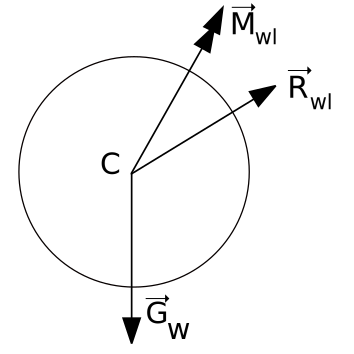
\includegraphics[scale=0.5]{Vrijlichaamsdiagram_wiel}
\caption{Het vrijlichaamsdiagram van het wiel}
\end{figure}

%\subsubsection*{Vrijlichaamsdiagram landingsgestel}
\begin{figure}[h!]
\centering
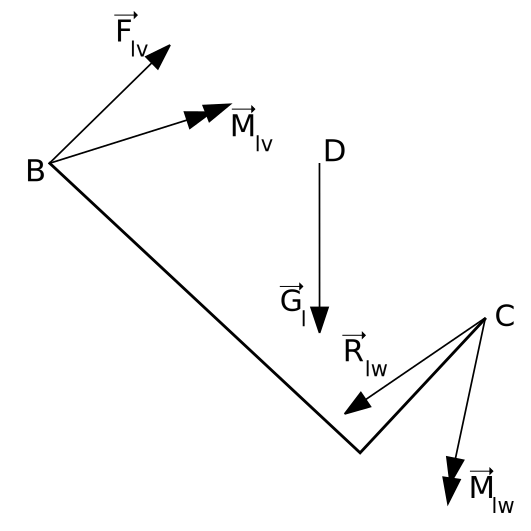
\includegraphics[scale=0.5]{Vrijlichaamsdiagram_landing}
\caption{Het vrijlichaamsdiagram van het landingsgestel}
\end{figure}

\subsection{Vraag 3}
Om de kracht op de vleugel door het landingsgestel te berekenen is het door een gebrek aan gegevens niet mogelijk om meteen de vleugel vrij te maken. Daar spelen te veel onbekende krachten op in. Het is wel mogelijk om de kracht van de vleugel op het landingsgestel te berekenen. Wegens de $3^{de}$ wet van Newton is deze gelijk aan de omgekeerde kracht van het landingsgestel op de vleugel.\
Het krachtenevenwicht van het landingsgestel is volledig bepaald als de kracht van het wiel op het landingsgestel bekend is. Het wiel wordt dus als eerste volledig vrijgemaakt.

\subsubsection{Het wiel}
OP het wiel werken twee krachten in, namelijk het gewicht en de kracht van het landingsgestel op het wiel. De som van deze twee krachten is gelijk aan de verandering van de impuls van het wiel.

\begin{equation*}
\overrightarrow{G_{w}}+\overrightarrow{R_{wl}}=\frac{d\overrightarrow{p_{w}}}{dt}
\end{equation*}

In een vorige opgave is de verandering van het impuls al eens berekend. Het gewicht wordt gegeven door de volgende formule.

\begin{equation*}
\overrightarrow{G_{w}}
=	\begin{bmatrix}
	0\\
	0\\
	-gm_{w}\
	\end{bmatrix}
\end{equation*}

De kracht $\overrightarrow{R_{wl}}$ wordt nu berekend en omgekeerd om de gewenste kracht $\overrightarrow{R_{lw}}$ te bekomen.


\subsubsection{Het landingsgestel}
Op het landingsgestel werken er drie krachten. De eerste kracht is natuurlijk het gewicht van het landingsgestel zelf. Vervolgens is er nog de kracht omwille van het wiel die in het vorige deel werd berekent en de kracht door de vleugel. Deze laatste kracht wordt berekend en omgedraaid om de gevraagde kracht te bekomen.

\begin{equation*}
\overrightarrow{G_{l}}+\overrightarrow{R_{lw}}+\overrightarrow{F_{lv}}=\frac{d\overrightarrow{p_{l}}}{dt}
\end{equation*}

Van deze termen is er maar \'e\'en onbekend, namelijk de kracht door de vleugel. De vergelijking wordt dus opgelost naar deze term en de oplossing wordt omgedraaid. Dit is de gevraagde kracht van het landingsgestel op de vleugel.

\subsection{Vraag 4}
Ook voor het berekenen van het moment van het landingsgestel op de vleugel zijn er niet genoeg gegevens om de vleugel direct vrij te maken. De $3¨{de}$ wet van Newton geldt ook voor momenten, dus dit laat toe om het moment van de vleugel op het landingsgestel te berekenen. Dit moment wordt vervolgens omgedraaid en dit resultaat is het gevraagde mometn. Op het landingsgestel werkt er echter nog een onbekend moment vanwege het wiel. De eerste stap bestaat dus uit het vrijmaken van het wiel en dit moment te bepalen.\\

Er speelt maar \'e\'en moment in op het wiel, namelijk het moment vanwege het landingsgestel. De krachten zorgen niet voor momenten aangezien ze aangrijpen in het massacentrum.

\begin{equation*}
\overrightarrow{M_{w,l}}=\frac{d\overrightarrow{L_{w,wereld}}}{dt}
\end{equation*}

Het moment van het wiel op het landingsgestel is gelijk aan het tegengestelde van dit moment.

\begin{equation*}
\overrightarrow{M_{l,w}}=-\overrightarrow{M_{w,l}}
\end{equation*}

Het momentenevenwicht van het landingsgestel rond het massacentrum is minder eenvoudig. De krachten op het landingsgestel vanwege het wiel en de vleugel zorgen voor een moment, dat gemakkelijk berekend kan worden. Er zijn ook twee vrije momenten, namelijk het moment door de vleugel en het moment door het wiel. Deze vergelijking wordt nu opgelost naar het moment door de vleugel.

\begin{equation*}
\overrightarrow{M_{l,v}}=\frac{d\overrightarrow{L_{l,wereld}}}{dt}-\left(-\overrightarrow{{r}_{D,C}}\times \overrightarrow{R_{l,w}}\right)-\left(-\overrightarrow{{r}_{D,B}}\times \overrightarrow{F_{l,v}} \right)-\overrightarrow{M_{l,w}}
\end{equation*}

\begin{equation*}
M_{v,l}=-M_{l,v}=\frac{dL_{l,wereld}}{dt}+\begin{bmatrix}
1/16\, \left( -2\,
\omega_{g}\,\omega_{i}\, \left( m_{l}+16\,m_{w} \right) {l_{4}}^{2}+6
\,l_{4}\,l_{3}\,\alpha_{g}\, \left( m_{l}+16/3\,m_{w} \right) +32\,
\omega_{g}\,\omega_{i}\, \left(  \left( {\frac {9\,m_{l}}{16}}+m_{w}
 \right) {l_{3}}^{2}+{\it I\_w\_xx}-{\it I\_w\_zz} \right)  \right) 
 \left( \cos \left( \beta \right)  \right) ^{2}+1/16\, \left(  \left( 
-\alpha_{g}\, \left( m_{l}+16\,m_{w} \right) {l_{4}}^{2}-12\,l_{4}\,
\omega_{i}\,l_{3}\, \left( m_{l}+16/3\,m_{w} \right) \omega_{g}+16\,
 \left(  \left( {\frac {9\,m_{l}}{16}}+m_{w} \right) {l_{3}}^{2}+{\it 
I\_w\_xx}-{\it I\_w\_zz} \right) \alpha_{g} \right) \sin \left( \beta
 \right) -12\,l_{3}\, \left( m_{l}+4/3\,m_{w} \right) g\sin \left( 
\alpha \right) -12\, \left( m_{l}+4/3\,m_{w} \right)  \left( l_{1}\,
\alpha_{g}+{\it a\_v} \right) l_{3}-16\,\alpha_{w}\,{\it I\_w\_xx}
 \right) \cos \left( \beta \right) +1/16\, \left( 4\,gl_{4}\, \left( m
_{l}+4\,m_{w} \right) \sin \left( \alpha \right) +4\, \left( m_{l}+4\,
m_{w} \right)  \left( l_{1}\,\alpha_{g}+{\it a\_v} \right) l_{4}-16\,
\omega_{i}\,\omega_{w}\, \left( {\it I\_w\_xx}-{\it I\_w\_yy}+{\it 
I\_w\_zz} \right)  \right) \sin \left( \beta \right) +1/8\,\omega_{g}
\,\omega_{i}\, \left( m_{l}+16\,m_{w} \right) {l_{4}}^{2}-3/16\,l_{4}
\,l_{3}\,\alpha_{g}\, \left( m_{l}+16/3\,m_{w} \right) -\omega_{g}\,
\omega_{i}\, \left( {\it I\_w\_xx}-{\it I\_w\_yy}-{\it I\_w\_zz}
 \right) \\
 %
 1/16\, \left(  \left( -9\, \left( m_{l}+
{\frac {16\,m_{w}}{9}} \right) \alpha_{g}\,{l_{3}}^{2}+12\,l_{4}\,
\omega_{i}\,l_{3}\, \left( m_{l}+16/3\,m_{w} \right) \omega_{g}-16\,
 \left(  \left( -m_{l}/16-m_{w} \right) {l_{4}}^{2}+{\it I\_w\_xx}-{
\it I\_w\_zz} \right) \alpha_{g} \right) \sin \left( \alpha \right) +6
\,\cos \left( \alpha \right)  \left( m_{l}+16/3\,m_{w} \right) l_{3}\,
{\omega_{g}}^{2}l_{4} \right)  \left( \cos \left( \beta \right) 
 \right) ^{2}+1/16\, \left(  \left(  \left( 18\, \left( m_{l}+{\frac {
16\,m_{w}}{9}} \right) \omega_{g}\,\omega_{i}\,{l_{3}}^{2}+6\,l_{4}\,l
_{3}\,\alpha_{g}\, \left( m_{l}+16/3\,m_{w} \right) +32\, \left( 
 \left( -m_{l}/16-m_{w} \right) {l_{4}}^{2}+{\it I\_w\_xx}-{\it 
I\_w\_zz} \right) \omega_{g}\,\omega_{i} \right) \sin \left( \beta
 \right) -4\, \left( m_{l}+4\,m_{w} \right)  \left( l_{1}\,\alpha_{g}+
{\it a\_v} \right) l_{4}+16\,\omega_{i}\,\omega_{w}\, \left( {\it 
I\_w\_xx}-{\it I\_w\_yy}+{\it I\_w\_zz} \right)  \right) \sin \left( 
\alpha \right) +16\, \left(  \left( {\frac {9\,m_{l}}{16}}+m_{w}
 \right) {l_{3}}^{2}+ \left( -m_{l}/16-m_{w} \right) {l_{4}}^{2}+{\it 
I\_w\_xx}-{\it I\_w\_zz} \right) \cos \left( \alpha \right) {\omega_{g
}}^{2}\sin \left( \beta \right) +16\,\omega_{g}\, \left( -3/4\,
 \left( m_{l}+4/3\,m_{w} \right) l_{3}\,l_{1}\,\omega_{g}+\omega_{w}\,
 \left( {\it I\_w\_yy}-{\it I\_w\_zz}+{\it I\_w\_xx} \right)  \right) 
\cos \left( \alpha \right) -4\,gl_{4}\, \left( m_{l}+4\,m_{w} \right) 
 \right) \cos \left( \beta \right) +1/16\, \left(  \left( -12\,
 \left( m_{l}+4/3\,m_{w} \right)  \left( l_{1}\,\alpha_{g}+{\it a\_v}
 \right) l_{3}-16\,\alpha_{w}\,{\it I\_w\_xx} \right) \sin \left( 
\beta \right) +9\, \left( m_{l}+{\frac {16\,m_{w}}{9}} \right) \alpha_
{g}\,{l_{3}}^{2}-6\,l_{4}\,\omega_{i}\,l_{3}\, \left( m_{l}+16/3\,m_{w
} \right) \omega_{g}+16\,\alpha_{g}\,{\it I\_w\_xx} \right) \sin
 \left( \alpha \right) +1/16\, \left( 4\,{\omega_{g}}^{2}l_{1}\,l_{4}
\, \left( m_{l}+4\,m_{w} \right) \cos \left( \alpha \right) -12\,l_{3}
\, \left( m_{l}+4/3\,m_{w} \right) g \right) \sin \left( \beta
 \right) -\cos \left( \alpha \right)  \left( {\frac {9\,\alpha_{i}\,{l
_{3}}^{2}}{16} \left( m_{l}+{\frac {16\,m_{w}}{9}} \right) }+3/16\,l_{
4}\,l_{3}\, \left( m_{l}+16/3\,m_{w} \right) {\omega_{g}}^{2}+ \left( 
 \left( m_{l}/16+m_{w} \right) {l_{4}}^{2}+{\it I\_w\_yy} \right) 
\alpha_{i} \right) \\ 
%
1/16\, \left(  \left( -12\,l_{
4}\,\omega_{i}\,l_{3}\, \left( m_{l}+16/3\,m_{w} \right) \omega_{g}-16
\,\alpha_{g}\, \left(  \left( -{\frac {9\,m_{l}}{16}}-m_{w} \right) {l
_{3}}^{2}+ \left( m_{l}/16+m_{w} \right) {l_{4}}^{2}+{\it I\_w\_zz}-{
\it I\_w\_xx} \right)  \right) \cos \left( \alpha \right) +6\,{\omega_
{g}}^{2}\sin \left( \alpha \right) l_{4}\,l_{3}\, \left( m_{l}+16/3\,m
_{w} \right)  \right)  \left( \cos \left( \beta \right)  \right) ^{2}+
1/16\, \left(  \left(  \left( 32\,\omega_{i}\, \left(  \left( -{\frac 
{9\,m_{l}}{16}}-m_{w} \right) {l_{3}}^{2}+ \left( m_{l}/16+m_{w}
 \right) {l_{4}}^{2}+{\it I\_w\_zz}-{\it I\_w\_xx} \right) \omega_{g}-
6\,l_{4}\,l_{3}\,\alpha_{g}\, \left( m_{l}+16/3\,m_{w} \right) 
 \right) \sin \left( \beta \right) +4\, \left( m_{l}+4\,m_{w} \right) 
 \left( l_{1}\,\alpha_{g}+{\it a\_v} \right) l_{4}+16\,\omega_{i}\,
\omega_{w}\, \left( {\it I\_w\_yy}-{\it I\_w\_zz}-{\it I\_w\_xx}
 \right)  \right) \cos \left( \alpha \right) +16\,\omega_{g}\,\sin
 \left( \alpha \right)  \left( -\omega_{g}\, \left(  \left( -{\frac {9
\,m_{l}}{16}}-m_{w} \right) {l_{3}}^{2}+ \left( m_{l}/16+m_{w}
 \right) {l_{4}}^{2}+{\it I\_w\_zz}-{\it I\_w\_xx} \right) \sin
 \left( \beta \right) -3/4\, \left( m_{l}+4/3\,m_{w} \right) l_{3}\,l_
{1}\,\omega_{g}+\omega_{w}\, \left( {\it I\_w\_yy}-{\it I\_w\_zz}+{
\it I\_w\_xx} \right)  \right)  \right) \cos \left( \beta \right) +1/
16\, \left(  \left( 12\, \left( m_{l}+4/3\,m_{w} \right)  \left( l_{1}
\,\alpha_{g}+{\it a\_v} \right) l_{3}+16\,\alpha_{w}\,{\it I\_w\_xx}
 \right) \sin \left( \beta \right) +6\,l_{4}\,\omega_{i}\,l_{3}\,
 \left( m_{l}+16/3\,m_{w} \right) \omega_{g}-9\,\alpha_{g}\, \left( 
 \left( m_{l}+{\frac {16\,m_{w}}{9}} \right) {l_{3}}^{2}+{\frac {16\,{
\it I\_w\_xx}}{9}} \right)  \right) \cos \left( \alpha \right) -
 \left( -1/4\,{\omega_{g}}^{2}l_{1}\,l_{4}\, \left( m_{l}+4\,m_{w}
 \right) \sin \left( \beta \right) +3/16\,l_{4}\,l_{3}\, \left( m_{l}+
16/3\,m_{w} \right) {\omega_{g}}^{2}+ \left(  \left( {\frac {9\,m_{l}
}{16}}+m_{w} \right) {l_{3}}^{2}+ \left( m_{l}/16+m_{w} \right) {l_{4}
}^{2}+{\it I\_w\_yy} \right) \alpha_{i} \right) \sin \left( \alpha
 \right) \
\end{bmatrix}
\end{equation*}

\subsection{Vraag 5}
Het moment dat door de vleugel op het landingsgestel wordt geleverd is gelijk aan het omgekeerde van het moment dat door het landingsgestel op de vleugel wordt geleverd.
%Dit moment wordt in feite niet volledig door de actuator geleverd. De actuator kan immers alleen maar een moment volgens de $y'$-as leveren. Dit zorgt er dus voor dat de actuator alleen voor moment met y- en z-co\"ordinaten kan zorgen.


\begin{align*}
M_{l,v}=\frac{dL_{l,wereld}}{dt}+\begin{bmatrix}
1/16\, \left( 2\,
\omega_{g}\,\omega_{i}\, \left( m_{l}+16\,m_{w} \right) {l_{4}}^{2}-6
\,l_{4}\,l_{3}\,\alpha_{g}\, \left( m_{l}+16/3\,m_{w} \right) -32\,
\omega_{g}\,\omega_{i}\, \left(  \left( {\frac {9\,m_{l}}{16}}+m_{w}
 \right) {l_{3}}^{2}+{\it I\_w\_xx}-{\it I\_w\_zz} \right)  \right) 
 \left( \cos \left( \beta \right)  \right) ^{2}+1/16\, \left(  \left( 
\alpha_{g}\, \left( m_{l}+16\,m_{w} \right) {l_{4}}^{2}+12\,l_{4}\,
\omega_{i}\,l_{3}\, \left( m_{l}+16/3\,m_{w} \right) \omega_{g}-16\,
 \left(  \left( {\frac {9\,m_{l}}{16}}+m_{w} \right) {l_{3}}^{2}+{\it 
I\_w\_xx}-{\it I\_w\_zz} \right) \alpha_{g} \right) \sin \left( \beta
 \right) +12\, \left( m_{l}+4/3\,m_{w} \right) l_{3}\,g\sin \left( 
\alpha \right) +12\, \left( l_{1}\,\alpha_{g}+{\it a\_v} \right) 
 \left( m_{l}+4/3\,m_{w} \right) l_{3}+16\,\alpha_{w}\,{\it I\_w\_xx}
 \right) \cos \left( \beta \right) +1/16\, \left( -4\,gl_{4}\, \left( 
m_{l}+4\,m_{w} \right) \sin \left( \alpha \right) -4\, \left( m_{l}+4
\,m_{w} \right)  \left( l_{1}\,\alpha_{g}+{\it a\_v} \right) l_{4}+16
\,\omega_{i}\,\omega_{w}\, \left( {\it I\_w\_xx}-{\it I\_w\_yy}+{\it 
I\_w\_zz} \right)  \right) \sin \left( \beta \right) -1/8\,\omega_{g}
\,\omega_{i}\, \left( m_{l}+16\,m_{w} \right) {l_{4}}^{2}+3/16\,l_{4}
\,l_{3}\,\alpha_{g}\, \left( m_{l}+16/3\,m_{w} \right) +\omega_{g}\,
\omega_{i}\, \left( {\it I\_w\_xx}-{\it I\_w\_yy}-{\it I\_w\_zz}
 \right) \\ 
 %
 1/16\, \left(  \left( 9\, \left( m_{l}+{
\frac {16\,m_{w}}{9}} \right) \alpha_{g}\,{l_{3}}^{2}-12\,l_{4}\,
\omega_{i}\,l_{3}\, \left( m_{l}+16/3\,m_{w} \right) \omega_{g}+16\,
 \left(  \left( -m_{l}/16-m_{w} \right) {l_{4}}^{2}+{\it I\_w\_xx}-{
\it I\_w\_zz} \right) \alpha_{g} \right) \sin \left( \alpha \right) -6
\,\cos \left( \alpha \right) l_{3}\,{\omega_{g}}^{2} \left( m_{l}+16/3
\,m_{w} \right) l_{4} \right)  \left( \cos \left( \beta \right) 
 \right) ^{2}+1/16\, \left(  \left(  \left( -18\,\omega_{g}\, \left( m
_{l}+{\frac {16\,m_{w}}{9}} \right) \omega_{i}\,{l_{3}}^{2}-6\,l_{4}\,
l_{3}\,\alpha_{g}\, \left( m_{l}+16/3\,m_{w} \right) -32\, \left( 
 \left( -m_{l}/16-m_{w} \right) {l_{4}}^{2}+{\it I\_w\_xx}-{\it 
I\_w\_zz} \right) \omega_{g}\,\omega_{i} \right) \sin \left( \beta
 \right) +4\, \left( m_{l}+4\,m_{w} \right)  \left( l_{1}\,\alpha_{g}+
{\it a\_v} \right) l_{4}-16\,\omega_{i}\,\omega_{w}\, \left( {\it 
I\_w\_xx}-{\it I\_w\_yy}+{\it I\_w\_zz} \right)  \right) \sin \left( 
\alpha \right) -16\, \left(  \left( {\frac {9\,m_{l}}{16}}+m_{w}
 \right) {l_{3}}^{2}+ \left( -m_{l}/16-m_{w} \right) {l_{4}}^{2}+{\it 
I\_w\_xx}-{\it I\_w\_zz} \right) \cos \left( \alpha \right) {\omega_{g
}}^{2}\sin \left( \beta \right) -16\, \left( -3/4\,l_{3}\,l_{1}\,
 \left( m_{l}+4/3\,m_{w} \right) \omega_{g}+\omega_{w}\, \left( {\it 
I\_w\_yy}-{\it I\_w\_zz}+{\it I\_w\_xx} \right)  \right) \omega_{g}\,
\cos \left( \alpha \right) +4\,gl_{4}\, \left( m_{l}+4\,m_{w} \right) 
 \right) \cos \left( \beta \right) +1/16\, \left(  \left( 12\, \left( 
l_{1}\,\alpha_{g}+{\it a\_v} \right)  \left( m_{l}+4/3\,m_{w} \right) 
l_{3}+16\,\alpha_{w}\,{\it I\_w\_xx} \right) \sin \left( \beta
 \right) -9\, \left( m_{l}+{\frac {16\,m_{w}}{9}} \right) \alpha_{g}\,
{l_{3}}^{2}+6\,l_{4}\,\omega_{i}\,l_{3}\, \left( m_{l}+16/3\,m_{w}
 \right) \omega_{g}-16\,\alpha_{g}\,{\it I\_w\_xx} \right) \sin
 \left( \alpha \right) +1/16\, \left( -4\,{\omega_{g}}^{2}l_{1}\,l_{4}
\, \left( m_{l}+4\,m_{w} \right) \cos \left( \alpha \right) +12\,
 \left( m_{l}+4/3\,m_{w} \right) l_{3}\,g \right) \sin \left( \beta
 \right) +\cos \left( \alpha \right)  \left( {\frac {9\,\alpha_{i}\,{l
_{3}}^{2}}{16} \left( m_{l}+{\frac {16\,m_{w}}{9}} \right) }+3/16\,l_{
4}\,l_{3}\, \left( m_{l}+16/3\,m_{w} \right) {\omega_{g}}^{2}+ \left( 
 \left( m_{l}/16+m_{w} \right) {l_{4}}^{2}+{\it I\_w\_yy} \right) 
\alpha_{i} \right) \\ 
%
1/16\, \left(  \left( 12\,l_{4
}\,\omega_{i}\,l_{3}\, \left( m_{l}+16/3\,m_{w} \right) \omega_{g}+16
\,\alpha_{g}\, \left(  \left( -{\frac {9\,m_{l}}{16}}-m_{w} \right) {l
_{3}}^{2}+ \left( m_{l}/16+m_{w} \right) {l_{4}}^{2}+{\it I\_w\_zz}-{
\it I\_w\_xx} \right)  \right) \cos \left( \alpha \right) -6\,{\omega_
{g}}^{2}\sin \left( \alpha \right) l_{4}\,l_{3}\, \left( m_{l}+16/3\,m
_{w} \right)  \right)  \left( \cos \left( \beta \right)  \right) ^{2}+
1/16\, \left(  \left(  \left( -32\,\omega_{i}\, \left(  \left( -{
\frac {9\,m_{l}}{16}}-m_{w} \right) {l_{3}}^{2}+ \left( m_{l}/16+m_{w}
 \right) {l_{4}}^{2}+{\it I\_w\_zz}-{\it I\_w\_xx} \right) \omega_{g}+
6\,l_{4}\,l_{3}\,\alpha_{g}\, \left( m_{l}+16/3\,m_{w} \right) 
 \right) \sin \left( \beta \right) -4\, \left( m_{l}+4\,m_{w} \right) 
 \left( l_{1}\,\alpha_{g}+{\it a\_v} \right) l_{4}-16\,\omega_{i}\,
\omega_{w}\, \left( {\it I\_w\_yy}-{\it I\_w\_zz}-{\it I\_w\_xx}
 \right)  \right) \cos \left( \alpha \right) -16\,\omega_{g}\,\sin
 \left( \alpha \right)  \left( -\omega_{g}\, \left(  \left( -{\frac {9
\,m_{l}}{16}}-m_{w} \right) {l_{3}}^{2}+ \left( m_{l}/16+m_{w}
 \right) {l_{4}}^{2}+{\it I\_w\_zz}-{\it I\_w\_xx} \right) \sin
 \left( \beta \right) -3/4\,l_{3}\,l_{1}\, \left( m_{l}+4/3\,m_{w}
 \right) \omega_{g}+\omega_{w}\, \left( {\it I\_w\_yy}-{\it I\_w\_zz}+
{\it I\_w\_xx} \right)  \right)  \right) \cos \left( \beta \right) +1/
16\, \left(  \left( -12\, \left( l_{1}\,\alpha_{g}+{\it a\_v} \right) 
 \left( m_{l}+4/3\,m_{w} \right) l_{3}-16\,\alpha_{w}\,{\it I\_w\_xx}
 \right) \sin \left( \beta \right) -6\,l_{4}\,\omega_{i}\,l_{3}\,
 \left( m_{l}+16/3\,m_{w} \right) \omega_{g}+9\,\alpha_{g}\, \left( 
 \left( m_{l}+{\frac {16\,m_{w}}{9}} \right) {l_{3}}^{2}+{\frac {16\,{
\it I\_w\_xx}}{9}} \right)  \right) \cos \left( \alpha \right) +
 \left( -1/4\,{\omega_{g}}^{2}l_{1}\,l_{4}\, \left( m_{l}+4\,m_{w}
 \right) \sin \left( \beta \right) +3/16\,l_{4}\,l_{3}\, \left( m_{l}+
16/3\,m_{w} \right) {\omega_{g}}^{2}+ \left(  \left( {\frac {9\,m_{l}
}{16}}+m_{w} \right) {l_{3}}^{2}+ \left( m_{l}/16+m_{w} \right) {l_{4}
}^{2}+{\it I\_w\_yy} \right) \alpha_{i} \right) \sin \left( \alpha
 \right) \
\end{bmatrix}
\end{align*}
\end{document}